\begin{figure}[htbp]\centering
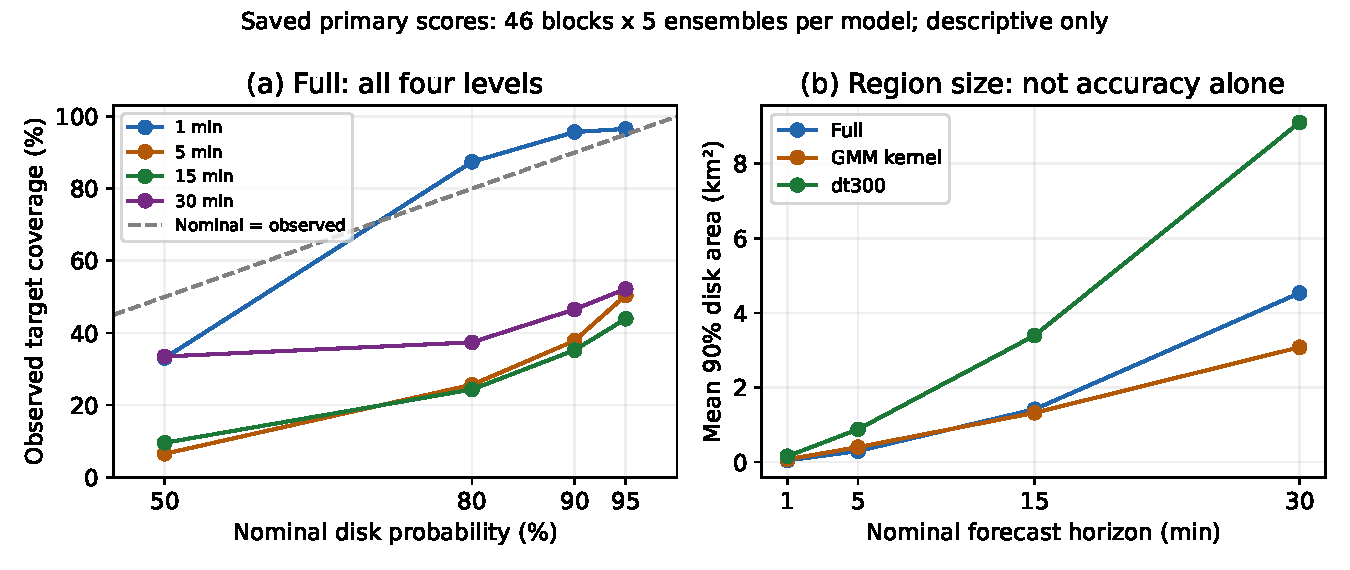
\includegraphics[width=\linewidth]{../figures/preliminary-calibration-area.pdf}
\caption{原46块、五种子汇总下的校准与大小。左为Full的16个覆盖值（四概率档乘四时域），
应接近对角线，而非曲线越高越好；右为三配置乘四时域的12个平均面积，必须与覆盖配读。
连线引导阅读，不增加中间时域或校准检验。}
\label{fig:reader-calibration}\end{figure}
\begin{table}[htbp]\centering
\caption{30分钟名义90\%圆：三配置、九个保存汇总值。每配置46块，各块五集合；
半径与面积分别平均，平均面积所对应的半径不是平均半径。}
\label{tab:reader-regions}
\begin{tabular}{lrrr}\toprule
模型 & 覆盖（\%） & 平均面积（km$^2$） & 平均半径（m）\\\midrule
Full01 & 46.52 & 4.534 & 1183.6\\
GMM & 45.22 & 3.079 & 989.5\\
dt300 & 64.35 & 9.109 & 1692.8\\\bottomrule
\end{tabular}\end{table}
dt300平均面积约为Full两倍，包含率仍低于名义90\%。区域扩大可以包含更多目标，
同时其中心位置反而更不准确；GMM区域较小也不能单独证明不确定性预测更好。
覆盖率在每块用五个模拟圆检查同一个真实目标；每时域有46个目标，不是230个独立目标。
块内五种子包含比例只能取0、20、40、60、80、100\%六档。补充块图的552点会在这些档位
重叠，块中位覆盖100\%或视觉密集都不是条件校准证明。
这些现象支持同时报告区域大小与包含率，并保留完整块摘要。
\FloatBarrier
